\documentclass[12pt,a4paper]{article}
\usepackage[utf8x]{inputenc}
\usepackage{ucs}
\usepackage{amsmath}
\usepackage{amsfonts}
\usepackage{amssymb}
\usepackage{graphicx}
\usepackage{grffile}
\usepackage{float}
\usepackage{multicol}
\usepackage[portuguese]{babel}
\title{Trabalho 2}
\author{André Garnier Coutinho}
\setlength{\textwidth}{17cm}
\setlength{\textheight}{24cm}
\addtolength{\topmargin}{-2cm}
\addtolength{\oddsidemargin}{-2cm}
\begin{document}
\begin{center}
\textbf{Escola Politécnica da USP\\
IC2014 - Grupo de pesquisa em Robótica e suas aplicações\\}
\end{center}

\begin{center}
\textbf{Cinemática 3D - Parte I}
\end{center}

\noindent{\bf Considerações Algelinísticas: \\}

\begin{itemize}



\item Matrizes de transformações lineares:

$$ [T(u)]_{C} = [T]_{B/C} [u]_{B}  $$
\linebreak

\item Composição de transformações lineares: 

$$ [T(u)]_{D} = [T]_{C/D} [T]_{B/C} [u]_{B} $$
$$ \therefore [T]_{B/D} = [T]_{C/D} [T]_{B/C} $$
\linebreak

\item Mudança de base:

$$ [u]_{C} = [I]_{B/C} [u]_{B} $$
\linebreak

\item Se as bases forem ortonormais:

$$ [I]_{C/B} = [I]_{B/C}^t = [I]_{B/C}^{-1}  $$
\linebreak

\item Construção da matriz de mudança de base:

$$ [I]_{B/can} = \Big[ [ \hat{i}  ']_{can} | [\hat{j} ']_{can} | [\hat{k} ']_{can} \Big] $$


Sendo $  \{ \hat{i}  , \hat{j} , \hat{k} \} $ os versores da base canônica e $  \{ \hat{i}' , \hat{j}' , \hat{k}' \}  $ os versores da base $B$.
\linebreak

\end{itemize}
\pagebreak

\noindent{\bf Cinemática de posição \\}

\begin{itemize}

\item Matrizes de rotação em torno dos eixos $x,y$ e $z$: \\

$$[I]_{B/can} =
\begin{bmatrix}
1 & 0 & 0 \\
0 & c\theta & -s\theta \\
0 & s\theta & c\theta
\end{bmatrix}
= R(\theta, x) $$

$$[I]_{B/can} =
\begin{bmatrix}
c\theta & -s\theta & 0 \\
s\theta & c\theta & 0 \\
0 & 0 & 1
\end{bmatrix}
= R(\theta, z) $$

$$[I]_{B/can} =
\begin{bmatrix}
c\theta & 0 & s\theta \\
0 & 1 & 0 \\
-s\theta & 0 & c\theta
\end{bmatrix}
= R(\theta, y) $$
\linebreak

\item Matrizes de transformação homogênea:

$$
\begin{bmatrix}
x_C \\
y_C \\
z_C \\
1
\end{bmatrix}
=
[H]_{B/C}
\begin{bmatrix}
x_B \\
y_B \\
z_B \\
1
\end{bmatrix}
$$

\item[i)] Rotação pura:

$$ [H]_{B/C} =
\begin{bmatrix}
[I]_{B/C} & 0_{3x1} \\
0_{1x3} & 1
\end{bmatrix}
$$

\item[ii)] Translação pura:

$$ [H]_{B/C} =
\begin{bmatrix}
I_{3x3} & \vec{d}_C \\
0_{1x3} & 1
\end{bmatrix}
$$

Sendo $\vec{d} =  \overrightarrow{CB}$

\item[iii)] Translação seguida de rotação:

$$ [H]_{B/C} =
\begin{bmatrix}
I_{3x3} & \vec{d}_C \\
0_{1x3} & 1
\end{bmatrix}
\begin{bmatrix}
[I]_{B/C} & 0_{3x1} \\
0_{1x3} & 1
\end{bmatrix}
=
\begin{bmatrix}
[I]_{B/C} & \vec{d}_C \\
0_{1x3} & 1
\end{bmatrix}
$$ \\

\end{itemize}
Vetor que equações de posição:

$$ \Phi(X, \Theta) = 0 $$ \\
As matrizes de transformação homogêneas são utilizadas para encontrarmos a relação das coordenadas $\Theta$ dos atuadores com as coordenadas cartesianas $X$ da plataforma (ou garra). Essas relações são dadas de forma genérica como um vetor de funções nulas $ \Phi(X, \Theta) = 0 $. \\



\noindent{\bf Exemplo 1 \\}

\begin{figure}[h!]
	\centering
	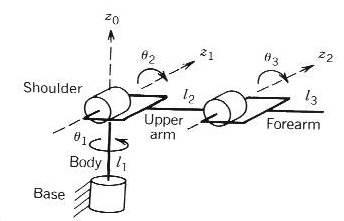
\includegraphics[scale=0.5]{RRR.jpg}  
	\caption{Mecanismo \underline{R}\underline{R}\underline{R}}
	\label{fig:figura1}
\end{figure}

Primeiro definimos um vetor $\Theta$ de coordenadas dos atuadores e um vetor $X$ das coordenadas da garra escritas no referencial inercial canônico:

\begin{multicols}{2}

$$ \Theta =
\begin{bmatrix}
\theta_1 \\
\theta_2 \\
\theta_3
\end{bmatrix} 
$$

$$ X =
\begin{bmatrix}
x_p \\
y_p \\
z_p
\end{bmatrix} 
$$

\end{multicols}

Depois disso, utilizamos as matrizes de transformação homogênea para estabelecer a relação das coordenadas $X$ com as coordenadas $\Theta$:

$$
\begin{bmatrix}
x_p \\
y_p \\
z_p \\
1
\end{bmatrix}
=
\begin{bmatrix}
c_1 & -s_1 & 0 & 0 \\
s_1 & c_1 & 0 & 0 \\
0 & 0 & 1 & h \\
0 & 0 & 0 & 1
\end{bmatrix}
\begin{bmatrix}
1 & 0 & 0 & 0  \\
0 & c_2 & -s_2 & 0 \\
0 & s_2 & c_2 & l_1 \\
0 & 0 & 0 & 1
\end{bmatrix}
\begin{bmatrix}
1 & 0 & 0 & 0 \\
0 & c_3 & -s_3 & l_2 \\
0 & s_3 & c_3 & 0 \\
0 & 0 & 0 & 1
\end{bmatrix}
\begin{bmatrix}
0 \\
l_3 \\
0 \\
1
\end{bmatrix}
$$

$$
\begin{bmatrix}
x_p \\
y_p \\
z_p \\
1
\end{bmatrix}
=
\begin{bmatrix}
c_1 & -s_1 c_{23} & s_1 s_{23} & -l_2 s_1 c_2 \\
s_1 & c_1 c_{23} & -c_1 s_{23} & l_2 c_1 c_2 \\
0 & s_{23} & c_{23} & h + l_1 + l_2 s_2 \\
0 & 0 & 0 & 1
\end{bmatrix}
\begin{bmatrix}
0 \\
l_3 \\
0 \\
1
\end{bmatrix}
$$

$$
\begin{bmatrix}
x_p \\
y_p \\
z_p \\
1
\end{bmatrix}
=
\begin{bmatrix}
-s_1 (l_2 c_2 + l_3 c_{23})  \\
c_1 (l_2 c_2 + l_3 c_{23}) \\
h + l_1 + l_2 s_2 + l_3 s_{23} \\
1
\end{bmatrix}
$$

Repare neste caso conseguimos isolar as coordenadas $X$ em função das coordenadas $\Theta$, ou seja: $X = f(\Theta)$. Sendo assim, o vetor de equações de posição é dado por $\Phi = X - f(\Theta)$. \\

\noindent{\bf Cinemática de velocidades \\}

$$ \frac{d}{dt} \Phi(X(t), \Theta(t)) = 0 $$
$$ \frac{\partial \Phi}{\partial X} \dot{X} + \frac{\partial \Phi}{\partial \Theta} \dot{\Theta} = 0 $$
$$ \therefore J_X \dot{X} + J_\Theta \dot{\Theta} = 0 $$

Como $J_X$ e $J_\Theta$ são funções apenas de $X$ e $\Theta$, tendo resolvido o problema de posição, o problema de velocidades torna-se um sistema linear. \\

\noindent{\bf Exemplo 2 \\}

O cinemática de velocidades para o mecanismo descrito no exemplo 1 é feita da seguinte maneira:

$$ J_X = \frac{\partial \Phi}{\partial X} = \frac{\partial}{\partial X} ( X - f(\Theta) ) = I = \begin{bmatrix}
1 & 0 & 0 \\
0 & 1 & 0 \\
0 & 0 & 1
\end{bmatrix} $$

$$ J_\Theta = \frac{\partial \Phi}{\partial \Theta} = \frac{\partial}{\partial \Theta} ( X - f(\Theta) ) = - \frac{\partial f}{\partial \Theta} = -\begin{bmatrix}
-c_1 (l_2 c_2 + l_3 c_{23}) & s_1 (l_2 s_2 + l_3 s_{23}) &  l_3 s_1 s_{23} \\
-s_1 (l_2 c_2 + l_3 c_{23}) & -c_1 (l_2 s_2 + l_3 s_{23}) & - l_3 c_1 s_{23} \\
0 & l_2 c_2 + l_3 c_{23} & l_3 c_{23}
\end{bmatrix}  $$

$$ \therefore \begin{bmatrix}
1 & 0 & 0 \\
0 & 1 & 0 \\
0 & 0 & 1
\end{bmatrix}
\begin{bmatrix}
\dot{x}_p \\
\dot{y}_p \\
\dot{z}_p
\end{bmatrix}
=
\begin{bmatrix}
-c_1 (l_2 c_2 + l_3 c_{23}) & s_1 (l_2 s_2 + l_3 s_{23}) &  l_3 s_1 s_{23} \\
-s_1 (l_2 c_2 + l_3 c_{23}) & -c_1 (l_2 s_2 + l_3 s_{23}) & - l_3 c_1 s_{23} \\
0 & l_2 c_2 + l_3 c_{23} & l_3 c_{23}
\end{bmatrix}
\begin{bmatrix}
\dot{\theta}_1 \\
\dot{\theta}_2 \\
\dot{\theta}_3
\end{bmatrix}
$$
\linebreak

\noindent{\bf Cinemática de acelerações \\}


$$  \frac{d}{dt} ( J_X \dot{X} + J_\Theta \dot{\Theta} ) = 0 $$
$$ \therefore \dot{J}_X \dot{X} + J_X \ddot{X} + \dot{J}_\Theta \dot{\Theta} + J_\Theta \ddot{\Theta} = 0  $$

Como $\dot{J}_X$ e $\dot{J}_\Theta$ são funções apenas de $X, \Theta, \dot{X}$ e $ \dot{\Theta} $, tendo resolvido os problemas de posição e velocidades, o problema de acelerações torna-se um sistema linear. \\

\noindent{\bf Exemplo 3 \\}

O cinemática de acelerações para o mecanismo descrito no exemplo 1 é feita da seguinte maneira:

$$ \dot{J}_X = 0 $$

$$ \dot{J}_\Theta = $$
$$ \begin{bmatrix}
s_1 (l_2 c_2 + l_3 c_{23}) & c_1 (l_2 s_2 + l_3 s_{23}) &  l_3 c_1 s_{23} \\
-c_1 (l_2 c_2 + l_3 c_{23}) & s_1 (l_2 s_2 + l_3 s_{23}) &  l_3 s_1 s_{23} \\
0 & 0 & 0
\end{bmatrix} \dot{\theta}_1 + $$

$$ \begin{bmatrix}
c_1 (l_2 s_2 + l_3 s_{23}) & s_1 (l_2 c_2 + l_3 c_{23}) &  l_3 s_1 c_{23} \\
s_1 (l_2 s_2 + l_3 s_{23}) & -c_1 (l_2 c_2 + l_3 c_{23}) & - l_3 c_1 c_{23} \\
0 & -l_2 s_2 - l_3 s_{23} & -l_3 s_{23}
\end{bmatrix} \dot{\theta}_2 + $$ 



$$ \begin{bmatrix}
l_3 c_1 s_{23} & l_3 s_1 c_{23} &  l_3 s_1 c_{23} \\
l_3 s_1   s_{23} & - l_3 c_1 c_{23} & - l_3 c_1 c_{23} \\
0 &  - l_3 s_{23} & - l_3 s_{23}
\end{bmatrix} \dot{\theta}_3 $$ 
\linebreak

\begin{center}
\textbf{Cinemática 3D - Parte II}
\end{center}

\noindent{\bf Considerações Algelinísticas: \\}

\begin{itemize}



\item Produto vetorial como um operador linear:

$$ \vec{\omega} \wedge \vec{v} = \begin{vmatrix}
\hat{i} & \hat{j} & \hat{k} \\
\omega_x & \omega_y & \omega_z \\
v_x & v_y & v_z
\end{vmatrix} 
= 
\begin{bmatrix}
\omega_y v_z - \omega_z v_y \\
\omega_z v_x - \omega_x v_z \\
\omega_x v_y - \omega_y v_x
\end{bmatrix}
=
\begin{bmatrix}
0 & - \omega_z & \omega_y \\
\omega_z & 0 & - \omega_x \\
- \omega_y & \omega_x & 0
\end{bmatrix}
\begin{bmatrix}
v_x \\
v_y \\
v_z
\end{bmatrix}
 $$
 
Ou seja, definindo:

$$ S(\vec{\omega}) = \begin{bmatrix}
0 & - \omega_z & \omega_y \\
\omega_z & 0 & - \omega_x \\
- \omega_y & \omega_x & 0
\end{bmatrix}
$$

Temos:

$$ \vec{\omega} \wedge \vec{v} = S(\vec{\omega}) \vec{v} $$

\item Mudança de base para matrizes de operadores lineares:

$$ [T]_B = [I]_{C/B} [T]_C [I]_{B/C} $$
\linebreak

\end{itemize}


\noindent{\bf Cinemática de velocidades angulares \\}
\linebreak

Como já foi visto anteriormente:

$$ [I]_{B/can} = \Big[ [ \hat{i}  ']_{can} | [\hat{j} ']_{can} | [\hat{k} ']_{can} \Big] $$


Sendo $  \{ \hat{i}  , \hat{j} , \hat{k} \} $ os versores da base canônica e $  \{ \hat{i}' , \hat{j}' , \hat{k}' \}  $ os versores da base $B$.

Derivando no tempo:

$$ [\dot{I}]_{B/can} = \Big[  [\vec{\omega}]_{can} \wedge [\hat{i}  ']_{can} | [\vec{\omega}]_{can} \wedge [\hat{j} ']_{can} | [\vec{\omega}]_{can} \wedge [\hat{k} ']_{can} \Big] $$
$$ = \Big[  [S(\vec{\omega})]_{can} [\hat{i}  ']_{can} | [S(\vec{\omega})]_{can}  [\hat{j} ']_{can} | [S(\vec{\omega})]_{can}  [\hat{k} ']_{can} \Big] $$
$$ = [S(\vec{\omega})]_{can} \Big[ [ \hat{i}  ']_{can} | [\hat{j} ']_{can} | [\hat{k} ']_{can} \Big] = [S(\vec{\omega})]_{can} [I]_{B/can}  $$
$$ \therefore [S(\vec{\omega})]_{can} = [\dot{I}]_{B/can} [I]_{B/can}^t  $$
\linebreak

Como $S(\vec{\omega})$ é um operador linear, podemos facilmente encontrar $[S(\vec{\omega})]_B$, se desejarmos:

$$ [S(\vec{\omega})]_B = [I]_{B/can}^t [S(\vec{\omega})]_{can} [I]_{B/can} = [I]_{B/can}^t [\dot{I}]_{B/can} [I]_{B/can}^t [I]_{B/can}   $$
$$ \therefore [S(\vec{\omega})]_B = [I]_{B/can}^t [\dot{I}]_{B/can} $$

\noindent{\bf Exemplo 4 \\}

Dertermine $[\vec{\omega}]_B$ da barra 3 do mecanismo do exemplo 1, sendo $B$ a base presa à barra 3. \\

Como já foi calculado anteriormente:

$$ [I]_{B/can} =
\begin{bmatrix}
c_1 & -s_1 c_{23} & s_1 s_{23}  \\
s_1 & c_1 c_{23} & -c_1 s_{23}  \\
0 & s_{23} & c_{23} 
\end{bmatrix}
$$

Derivando no tempo:

$$ [\dot{I}]_{B/can} =
\begin{bmatrix}
-s_1 & -c_1 c_{23} & c_1 s_{23}  \\
c_1 & -s_1 c_{23} & s_1 s_{23}  \\
0 & 0 & 0 
\end{bmatrix}
\dot{\theta}_1 +
\begin{bmatrix}
0 & s_1 s_{23} & s_1 c_{23}  \\
0 & -c_1 s_{23} & -c_1 c_{23}  \\
0 & c_{23} & -s_{23} 
\end{bmatrix}
(\dot{\theta}_2 + \dot{\theta}_3)
$$

$$ [S(\vec{\omega})]_B = 
\begin{bmatrix}
c_1 & s_1 & 0  \\
-s_1 c_{23} & c_1 c_{23} &  s_{23}  \\
s_1 s_{23} & -c_1 s_{23} & c_{23} 
\end{bmatrix} \Big\{
\begin{bmatrix}
-s_1 & -c_1 c_{23} & c_1 s_{23}  \\
c_1 & -s_1 c_{23} & s_1 s_{23}  \\
0 & 0 & 0 
\end{bmatrix}
\dot{\theta}_1 +
\begin{bmatrix}
0 & s_1 s_{23} & s_1 c_{23}  \\
0 & -c_1 s_{23} & -c_1 c_{23}  \\
0 & c_{23} & -s_{23} 
\end{bmatrix}
(\dot{\theta}_2 + \dot{\theta}_3)
\Big\}
 $$
 
 $$ [S(\vec{\omega})]_B = 
\begin{bmatrix}
0 & - c_{23} &  s_{23}  \\
c_{23} & 0 & 0 \\
-s_{23} & 0 & 0 
\end{bmatrix}
\dot{\theta}_1 +
\begin{bmatrix}
0 & 0 & 0  \\
0 & 0 & -1  \\
0 & 1 & 0 
\end{bmatrix}
(\dot{\theta}_2 + \dot{\theta}_3)
$$

$$ \therefore [\vec{\omega}]_B =
\begin{bmatrix}
\dot{\theta}_2 + \dot{\theta}_3 \\
s_{23} \dot{\theta}_1 \\
c_{23} \dot{\theta}_1
\end{bmatrix} $$


\end{document}
